\documentclass[border=6pt]{standalone}
\usepackage{tikz}
\begin{document}
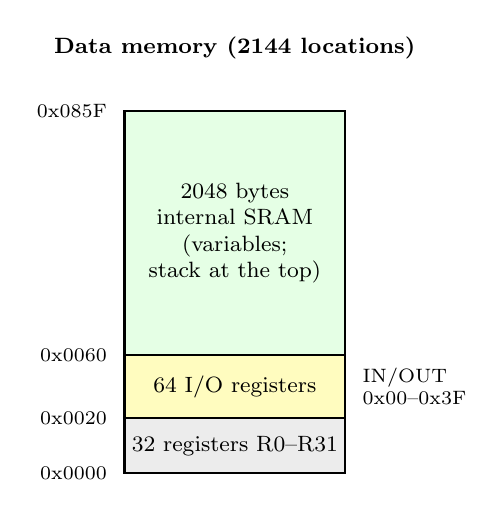
\begin{tikzpicture}[font=\small]
% Data memory
\begin{scope}
\node[font=\footnotesize\bfseries] at (1.4,5.4) {Data memory (2144 locations)};
\draw[thick,fill=gray!15] (0,0) rectangle (2.8,0.7);
\draw[thick,fill=yellow!25] (0,0.7) rectangle (2.8,1.5);
\draw[thick,fill=green!10] (0,1.5) rectangle (2.8,4.6);
\node[font=\footnotesize,align=center] at (1.4,0.35) {32 registers R0--R31};
\node[font=\footnotesize,align=center] at (1.4,1.1) {64 I/O registers};
\node[font=\footnotesize,align=center] at (1.4,3.05) {2048 bytes\\internal SRAM\\(variables;\\stack at the top)};
\foreach \y/\a in {0/0x0000,0.7/0x0020,1.5/0x0060,4.6/0x085F} \node[font=\scriptsize,anchor=east] at (-0.1,\y) {\a};
\node[font=\scriptsize,anchor=west,align=left] at (2.9,1.1) {IN/OUT\\0x00--0x3F};
\end{scope}
\end{tikzpicture}
\end{document}
